\chapter{Анализ литературы}


	\setcounter{subsection}{-1}
	\section{Технологии Интернета вещей}
	IoT включает в себя бесчисленное количество технологий и решений, и чтобы понять их все, необходимо
	потратить немало времени. Однако в целях упрощения существует возможность разбить весь IoT стек на
	четыре базовых технологических уровня, которые позволяют функционировать всему Интернету вещей.
	
	\textbf{Аппаратное обеспечение} устройств является первым из этих уровней. Устройства $-$ это те самые
	<<вещи>> в аббревиатуре IoT. Выступая в роли интерфейса между реальным и цифровым миром, они
	могут принимать разные формы и размеры, а также иметь разные уровни технологической оснащённости в
	зависимости от выполняемой задачи. Практически любой предмет может быть подключен к Интернету и
	оснащён необходимым инструментарием (сенсорами, датчиками и т.д.) в целях измерения и сбора данных.
	Единственным существенным ограничением может быть реальный практический сценарий использования.
	
	\textbf{Программное обеспечение} является элементом, который делает девайсы по-настоящему <<умными>>.
	Программы ответственны за коммуникацию с облаком, сбор данных, взаимодействие между устройствами,
	а также анализ данных в реальном времени. Более того, программное обеспечение помогает взаимодействовать
	с IoT системами на уровне приложения конечному пользователю, визуализируя обработанные данные для него.
	
	\textbf{Уровень коммуникации (уровень сообщения)} тесно связан с программным и аппаратным обеспечением, однако
	важно рассматривать его отдельно. Этот уровень содержит средства для обмена
	информацией между умными устройствами и остальным IoT миром. Он включает в себя как физическое соединение,
	так и специальные протоколы, на которых будет сделан акцент в данной работе. Выбор правильного решения
	для обмена сообщениями является ключевым при построении каждой системы. Технологии отличаются в
	зависимости от способа передачи данных и управления устройствами.
	
	Благодаря программному и аппаратному обеспечению девайсы могут считывать, что происходит вокруг, и
	коммуницировать с пользователями по специальным каналам связи. \textbf{IoT платформа} $-$ это место, в котором
	все собранные данные обрабатываются, анализируются и представляются пользователю в удобном виде.
	Её достоинством является извлечение полезных данных из большого объёма информации, который передаётся
	от устройств по каналам связи.
	
	
	\section{Используемые протоколы}
	
	Существует множество разнообразных способов взаимодействия умных устройств между собой. Поэтому
	при выборе протоколов для Интернета вещей часто возникает вопрос о том, есть ли реальная необходимость
	разработки новых решений, в то время как хорошо зарекомендовавшие себя протоколы сети Интернет уже
	используются повсеместно десятилетиями. Причина для этого кроется в том, что существующие протоколы
	часто оказываются недостаточно эффективными и слишком энергоёмкими для работы с возникающими
	IoT технологиями. Поэтому речь пойдёт об альтернативных решениях, посвящённых именно IoT системам.
	
	Одна из возможных классификаций разбивает все протоколы на три группы: ближнего, среднего и дальнего
	действия. Наиболее ярким представителем первой группы является Bluetooth, который несмотря на свою
	повсеместную распространённость остаётся далеко не лучшим решением, особенно при передаче больших
	объёмов данных. К последней группе относят такие протоколы как NB-IoT, LoRaWAN и SigFox.
	Эти решения являются весьма современными и продвинутыми, однако используются часто в масштабах
	предприятий. Наша же цель заключается в изучении решений, применимых к простым пользователям 
	IoT систем, поэтому данный раздел будет преимущественно сконцентрирован вокруг второй группы, 
	а именно протоколов средней зоны действия.
	
	Однако для полноты картины посмотрим вначале на протоколы ближнего и дальнего действия.
	
    \subsection{Bluetooth}
    
    Bluetooth – это стандарт беспроводной связи, предназначенный для обмена информацией на небольших 
    расстояниях между мобильными и некоторыми другими типами устройств. Этот стандарт описан в
    спецификации IEEE 802.15.1. Первая версия Bluetooth 1.0 была выпущена в 1998 году. Начиная с версии
    Bluetooth 4.2 (2014 год) было заявлено о поддержке IoT, а Bluetooth 5 и вовсе позиционируется как одна
    из лидирующих технологий в среде IoT. Однако у неё есть свои нюансы. До версии 5.0 главным из них 
    было малое количество устройств, способных объединяться в одну сеть. Оно ограничивалось лишь 8-ю узлами.
    Но в последних версиях этот показатель был увеличен на порядок. На данный момент максимальное количество
    устройств в Bluetooth-сети составляет 32767.
    
    Bluetooth функционирует в частотах от 2,4 до 2,485 ГГц. Дальность действия в 5-й версии составляет 40 метров,
    а скорость передачи данных $-$ до 2 Mbit/s. Была проведена существенная работа над энергопотреблением 
    устройств. А кроме того в последней версии заявлено о поддержке ячеистой топологии сети (более подробно
    о ней в разделе о ZigBee), что в будущем, при появлении большего количество устройств на новых версиях,
    позволит технологии как минимум сравниться по популярности и сценариям использования с другими
    стандартами, такими как ZigBee, Z-Wave и Wi-Fi.
    
    
    \subsection{Протоколы дальнего действия}
    
   	Рассмотрим лишь некоторые, самые популярные решения.
   	
   	\begin{itemize}
   		\item NarrowBand-IoT. Это новый стандарт радио технологий, который обеспечивает экстремально
   		низкое энергопотребление устройств (до 10 лет от одной батареи). Кроме того, он использует уже
   		существующую инфраструктуру сетей сотовой связи, что обеспечивает глобальное покрытие и
   		гарантированное качество сигнала.
   		\item LoRaWAN. Расшифровывается как Long Range Wide-Area Networking. Он заточен под
   		низкое энергопотребление и поддерживает огромные сети с миллионами устройств. Используется
   		в масштабах умных городов. Типичными примером может послужить дистанционное считывание 
   		показаний счётчиков электроэнергии и водоснабжения в многоквартирных домах.
   		\item SigFox. Технология обеспечивает простую и быструю связь между сенсорными устройствами 
   		в пределах беспроводной сети. Характеризуется ещё более низким энергопотреблением (до 20 лет
   		от одной батарее), однако имеет зависимость от существующей сотовой инфраструктуры.
   	\end{itemize}
   
   Поскольку перечисленные протоколы сильно отличаются по своим характеристикам от протоколов 
   ближнего и среднего действия, имеет смысл сравнить их отдельно в приведенной ниже таблице.
   
   \begin{table}[h]
   	\centering
   	\begin{tabular}{ | l | l | l | l |}
   		\hline
   		& NB-IoT & LoRaWAN & Sigfox \\ \hline
   		Скорость передачи & 100 Kbit/s & 50 Kbit/s & 100 bit/s \\ \hline
   		Энергопотребление & Низкое & Низкое & Низкое \\ \hline
   		Частота & < 1 GHz  & 150 MHz - 1 GHz & 900 MHz \\ \hline
   		Топология сети & Звезда & Звезда & Звезда \\
   		\hline
   	\end{tabular}
   	\caption{Сравнение протоколов дальнего действия}
   	\label{table-long-range-solutions}
   \end{table}
	

	\subsection{ZigBee}
	ZigBee $-$ это один из протоколов верхнего уровня, используемый в домашней автоматизации и других
	сферах IoT, построенный на базе стандарта IEEE 802.15.4. Он поддерживает высокую отказоустойчивость, 
	низкое энергопотребление, безопасность и надёжность.
	
	Протокол ZigBee описывает беспроводные персональные сети (Wireless personal area network, WPAN).
	Индивидуальные устройства в подобной сети могут работать на одной батарее до двух лет.
	Сети на основе ZigBee характеризуются довольно низкой пропускной способностью (до 250 Кбит/с) и
	дальностью связи между узлами до 100 метров. Протокол был задуман в 1998 году. Первоначальная 
	спецификация была признана стандартом IEEE в 2003 году, а первые модули, совместимые с ZigBee, 
	появились в массовой продаже в начале 2006 года \cite{zigbee-certified-products}.
	
	Существует три типа устройств ZigBee:
	
	\begin{enumerate}
		\item Координатор ZigBee (ZigBee Coordinator, ZC). Каждая сеть ZigBee должна иметь один координатор,
		который управляет всей сетью. Координатор выполняет функцию <<центра доверия>> (Trust Center, TC),
		обеспечивая генерацию, хранение и распространение ключей безопасности. Он отвечает за создание сети
		путём выбора наиболее свободного канала для коммуникации устройств. После этого координатор 
		разрешает другим устройствам присоединяться к сети и покидать её, ведя учёт всех устройств в сети.
		ZigBee координатор не может находиться в спящем режиме и должен быть непрерывно подключён
		к источнику питания.
		\item Маршрутизатор ZigBee (ZigBee Router, ZR). Маршрутизатор выступает в качестве промежуточного
		звена между координатором и конечными устройства. Сперва он должен получить разрешение на
		присоединение к сети от координатора, а после может перенаправлять трафик между устройствами и 
		позволять новым устройствам подключаться к сети. По аналогии с координатором маршрутизатор не
		может находиться в спящем режиме. Является опциональным устройством в сети.
		\item Конечное устройство ZigBee (ZigBee End Device, ZED). Это самый простой тип устройств в сети
		ZigBee. Обычно они питаются от батарее. Потребитель чаще всего знаком именно с этим типом
		устройства, к которому относятся, например, умные лампочки или датчики движения. Они содержат 
		достаточно функций, чтобы общаться с координатором или маршрутизатором, но не могут передавать 
		данные от других устройств. Такое взаимодействие позволяет узлу находиться в спящем режиме 
		значительную часть времени, что обеспечивает длительность автономной работы. ZED требует 
		наименьшего объёма памяти, поэтому является более дешёвым в производстве, чем координатор 
		или маршрутизатор.
	\end{enumerate}

	\begin{table}[h]
		\centering
		\begin{tabular}{ | p{9cm} | p{1cm} | p{1cm} | p{1cm} | }
			\hline
			& ZC & ZR & ZED \\ \hline
			Создание сети ZigBee & x &  &  \\ \hline
			Разрешение на присоединение к сети другим устройствам & x & x &  \\ \hline
			Назначение 16-битного сетевого адреса & x & x &  \\ \hline
			Обнаружение и запись путей для эффективной доставки сообщений & x & x &  \\ \hline
			Маршрутизация сетевых пакетов & x & x & x \\ \hline
			Присоединение и выход из сети & x & x & x \\ \hline
			Режим сна & & & x \\ \hline
		\end{tabular}
		\caption{Типы устройств ZigBee}
		\label{table-ZigBee-device-types}
	\end{table}
	
	ZigBee был разработан как стандарт для радиосетей с ячеистой (mesh) топологией.
	Кроме того, ZigBee поддерживает сети с топологией <<звезда>> и <<дерево>>. В каждой 
	сети должно быть одно устройство-координатор. В сетях с топологией <<звезда>> координатор должен 
	быть центральным узлом. Как древовидные, так и ячеистые сети позволяют использовать маршрутизаторы 
	ZigBee для расширения связи на сетевом уровне. Благодаря этому, используя несколько координаторов,
	дальность соединения может быть намного более базовых 100 метров. А за счёт построения оптимального
	маршрута в сетях с ячеистой топологии сеть в некоторых случаях может продолжать работу даже
	при выходе их строя одного из координаторов. \newline
	
	\begin{figure}[h]
		\centering
		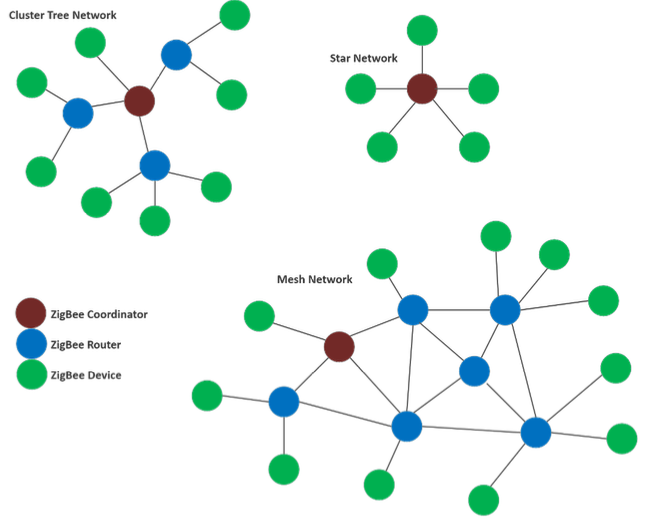
\includegraphics[scale=0.6]{resources/ZigBee-network-topologies}
		\caption{Топологии сети ZigBee}
		\label{fig1.1}
	\end{figure}

	Архитектура протокола состоит их четырёх уровней:
	
	\begin{enumerate}
		\item Физический (PHY). Физический уровень относится к стандарту IEEE 802.15.4. Этот уровень
		является ответственным за передачу битов информации путём отправки и получения пакетов
		данных, а также за выбор канала (и, соответственно, частоты).
		\item MAC (Medium Access Control). MAC $-$ ещё один уровень, относящийся к стандарту IEEE 802.15.4.
		Он служит интерфейсом между физическим и сетевым уровнями. MAC обеспечивает механизмы
		адресации и управления доступом к каналам.
		\item Сетевой (NWK). Этот уровень определяется уже ZigBee-спецификацией. Он ответственен
		в первую очередь за выбор топологии сети. После выбора канала координатор назначает каждому
		присоединяющемуся к сети устройству специальный идентификатор $-$ PAN ID (Personal Area Network ID).
		Этот идентификатор (16-битное число) используется для логического отделения узлов одной сети 
		ZigBee от узлов другой. На сетевом уровне также устанавливается адрес каждого узла в сети.
		\item Прикладной (APL). Прикладной уровень (или уровень Приложения) включает несколько
		подуровней. Application Support Sublayer (APS) предоставляет программный интерфейс между 
		уровнем NWK и приложениями, которые могут работать на устройстве. Именно он отвечает за
		безопасность всего прикладного уровня. ZigBee Device Object (ZDO) определяет, будет ли устройство
		координатором или конечным устройством. Application Framework является окружением для
		приложений ZigBee. Он определяется вендором, реализующим спецификацию, однако в последнее
		время много усилий направлено на совместимость устройств от различных производителей.
	\end{enumerate}

	Таким образом, ZigBee $-$ это спецификация протоколов APS (прикладного) и NWK (сетевого) уровней,
	использующих сервисы нижних уровней (MAC и PHY), регламентированных стандартом IEEE 802.15.4. \newline
	
	\begin{figure}[H]
		\centering
		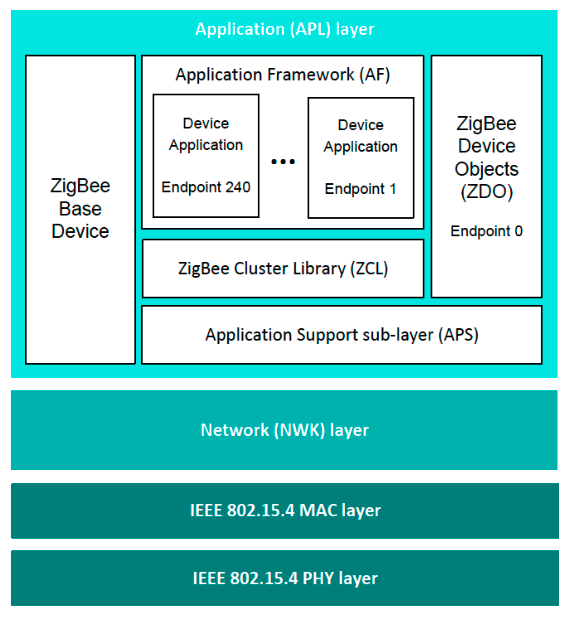
\includegraphics[scale=0.6]{resources/ZigBee-network-layers}
		\caption{Сетевые уровни ZigBee}
		\label{fig1.2}
	\end{figure}
	
   Типичные сферы применения протокола:
	\begin{itemize}
		\item домашняя автоматизация;
		\item промышленные системы управления;
		\item сбор медицинских данных;
		\item оповещение о задымлении и несанкционированном проникновении;
		\item автоматизация зданий.
	\end{itemize}

	ZigBee Alliance $-$ это группа компаний, которые поддерживают и публикуют стандарт ZigBee
	 \cite{zigbee-alliance}. Название 
	ZigBee является зарегистрированной торговой маркой этой группы и представляет собой не просто 
	технический стандарт. Организация публикует материалы, которые позволяют производителям 
	создавать совместимые продукты. Связь между IEEE 802.15.4 и ZigBee похожа на связь между 
	IEEE 802.11 и Wi-Fi Alliance. За годы существования альянса его членами стали более 500 компаний.
	
	
	\subsection{Z-Wave}
	Z-Wave $-$ это протокол беспроводной связи, используемый в основном для домашней автоматизации. 
	Он применяется преимущественно для управления бытовой техникой и другими устройствами, такими 
	как освещение, охранные системы, термостаты, окна, замки, бассейны и открыватели гаражных дверей.
	Как и другие протоколы, предназначенные для рынка автоматизации дома и офиса, система Z-Wave может 
	управляться через Интернет со смартфона, планшета или компьютера, а также локально через умную 
	колонку или хаб, настенную панель со шлюзом Z-Wave или центральным устройством управления. 
	Z-Wave обеспечивает совместимость на прикладном уровне между системами управления домом различных 
	производителей, входящих в её альянс. Число совместимых продуктов Z-Wave значительно растёт, 
	к 2019 году их количество составляло более 2600 \cite{z-wave-certified-products}.
	
	Протокол Z-Wave был разработан датской компанией Zensys, расположенной в Копенгагене, 
	в 1999 году. В этом же году была представлена потребительская 
	систему управления светом. Набор микросхем серии 100 был выпущен в 2003 году, а серии 200 $-$ 
	в мае 2005 года. Микросхема серии 500, также известная как Z-Wave Plus, была выпущена в марте 2013 года,
	с увеличенным в четыре раза объёмом памяти, улучшенным радиусом действия беспроводной связи и 
	увеличенным временем автономной работы. Технология начала распространяться в Северной Америке 
	примерно в 2005 году, когда пять компаний приняли Z-Wave и сформировали Z-Wave Alliance, целью 
	которого является продвижение использования технологии Z-Wave \cite{z-wave-alliance}. При этом 
	все продукты компаний, входящих в альянс, должны быть совместимы. В том же 2005 году технология
	получила первые инвестиции.
	
	В настоящее время Z-Wave Alliance насчитывает более 700 производителей. Основными членами альянса 
	являются ADT Corporation, Assa Abloy, Jasco, Leedarson, LG Uplus, Nortek Security \& Control, Ring, Silicon Labs, 
	SmartThings, Trane Technologies и Vivint.
	
	Взаимодействие Z-Wave на уровне приложений обеспечивает обмен информацией между устройствами 
	и позволяет всем аппаратным и программным средствам Z-Wave работать вместе. Технология беспроводной 
	ячеистой сети (аналогичная с ZigBee) позволяет любому узлу напрямую или косвенно общаться с соседними 
	узлами, управляя любыми дополнительными узлами. Узлы, находящиеся в радиусе действия, общаются друг 
	с другом напрямую. Если они не находятся в радиусе действия, они могут связаться с другим узлом, 
	который расположен в зоне действия обоих узлов, чтобы получить доступ и обменяться информацией.
	
	Z-Wave разработан для обеспечения надёжной передачи небольших пакетов данных с низкой задержкой 
	на скорости до 100 кбит/с. Пропускная способность составляет 40 кбит/с и подходит для приложений 
	управления и датчиков, в отличие от Wi-Fi и других систем беспроводных локальных сетей на базе IEEE 802.11, 
	которые предназначены в основном для высокой скорости передачи данных. Расстояние связи между 
	двумя узлами составляет около 40 метров.
	
	Z-Wave функционирует в диапазоне частот до 1 ГГц. Этот диапазон конкурирует с некоторыми беспроводными 
	телефонами и другими устройствами бытовой электроники, но позволяет избежать помех в виде Wi-Fi, Bluetooth 
	и других систем, работающих в переполненном диапазоне 2,4 ГГц.
	
	Z-Wave использует архитектуру ячеистой сети с маршрутизацией от источника. Устройства могут 
	связываться друг с другом, используя промежуточные узлы для активной маршрутизации и обхода 
	бытовых препятствий или мертвых зон. Таким образом, сеть Z-Wave может охватывать гораздо большее 
	расстояние, чем радиус действия одного узла. Однако при наличии нескольких таких переходов может 
	возникнуть небольшая задержка между управляющей командой и желаемым результатом.
	
	Простейшая сеть представляет собой одно управляемое устройство и первичный контроллер. Дополнительные 
	устройства могут быть добавлены в любое время, как и вторичные контроллеры, включая приложения 
	для смартфонов и ПК, разработанные для управления и контроля сети Z-Wave. Сеть может включать 
	до 232 устройств, а при необходимости увеличения количества устройств возможно объединение сетей.
	
	Каждой сети Z-Wave назначается идентификатор, а каждое устройство содержит идентификатор узла. 
	Идентификатор сети (Home ID) $-$ это общая идентификация всех узлов, принадлежащих к одной логической 
	сети Z-Wave. Сетевой ID имеет длину 4 байта и присваивается каждому устройству первичным контроллером, 
	когда устройство добавляется в сеть. Узлы с разными сетевыми идентификаторами не могут взаимодействовать 
	друг с другом. Идентификатор узла $-$ это адрес одного узла в сети. Идентификатор узла имеет 
	длину 1 байт и является уникальным в своей сети.
	
	Чип Z-Wave оптимизирован для устройств, работающих от батарей, и большую часть времени находится 
	в режиме энергосбережения, чтобы потреблять меньше энергии, просыпаясь только для выполнения своей 
	функции. В ячеистых сетях Z-Wave каждое устройство в доме распространяет беспроводные сигналы по 
	всему дому, что приводит к низкому энергопотреблению, позволяя устройствам работать годами без 
	необходимости замены батарей. Чтобы устройства Z-Wave могли передавать сторонние сообщения, 
	они не должны быть в спящем режиме. Поэтому устройства, работающие от батарей, не предназначены для 
	использования в качестве ретрансляторов.
	
	
	\subsection{Wi-Fi}
	Построенный на базе стандарта IEEE 802.11, Wi-Fi остаётся самым распространённым и наиболее
	известным беспроводным протоколом взаимодействия. Его широкое использование в мире IoT в
	основном ограничено энергопотреблением выше среднего по причине удержание качественного сигнала
	и быстрой передачи данных для лучшего соединения и надёжности. Несмотря на это Wi-Fi является
	ключевой технологией в развитии и распространении IoT.
	
	Для создания сети Wi-Fi требуются устройства, способные передавать беспроводные сигналы, то есть 
	такие устройства, как телефоны, компьютеры или маршрутизаторы. В домашних условиях маршрутизатор 
	используется для передачи интернет-соединения из общественной сети в частную домашнюю или офисную 
	сеть. Wi-Fi обеспечивает подключение к Интернету близлежащих устройств, находящихся в определенном 
	радиусе действия. Другой способ использования Wi-Fi $-$ создание точки доступа.
	
	Wi-Fi использует радиоволны, которые передают информацию на определенных частотах. Двумя основными
	частотами являются 2,4 ГГц и 5 ГГц. Оба частотных диапазона имеют ряд каналов, по которым могут 
	работать различные беспроводные устройства, что помогает распределить нагрузку таким образом, 
	чтобы индивидуальные соединения устройств не прерывались. Это в значительной степени предотвращает 
	переполнение беспроводных сетей.
	
	Диапазон в 100 метров является типичным для стандартного Wi-Fi соединения. Однако чаще всего радиус 
	действия ограничивается 10-35 метрами. На эффективное покрытие влияет мощность антенны 
	и частота передачи. Дальность и скорость Wi-Fi подключения к Интернету зависит от окружающей среды 
	и от того, обеспечивает ли оно внутреннее или внешнее покрытие.
	
	Технология Wi-Fi была создана в 1998 году. В 2018 году Wi-Fi Alliance \cite{wi-fi-alliance} ввёл упрощенную 
	нумерацию поколений Wi-Fi для обозначения оборудования, поддерживающего Wi-Fi 4 (802.11n), 
	Wi-Fi 5 (802.11ac) и Wi-Fi 6 (802.11ax). Эти поколения имеют высокую степень обратной совместимости 
	с предыдущими версиями. Альянс заявил, что уровень поколения 4, 5 или 6 может быть указан в 
	пользовательском интерфейсе при подключении, наряду с уровнем сигнала.
	
	\begin{table}[h]
		\centering
		\begin{tabular}{ | l | l | l | l | l | }
			\hline
			Поколение & Стандарт IEEE & Частота & Скорость передачи & Год \\ \hline
			Wi-Fi 0 & 802.11 & 2.4 GHz & 2 Mbit/s & 1997 \\ \hline
			Wi-Fi 1 & 802.11b & 2.4 GHz & 11 Mbit/s & 1999 \\ \hline
			Wi-Fi 2 & 802.11a & 5 GHz & 54 Mbit/s & 1999 \\ \hline
			Wi-Fi 3 & 802.11g & 2.4 GHz & 54 Mbit/s & 2003 \\ \hline
			Wi-Fi 4 & 802.11n & 2.4/5 GHz & 600 Mbit/s & 2008 \\ \hline
			Wi-Fi 5 & 802.11ac & 5 GHz & 6933 Mbit/s & 2014 \\ \hline
			Wi-Fi 6 & 802.11ax & 2.4/5 GHz & 9608 Mbit/s & 2019 \\ \hline
			Wi-Fi 6E & 802.11ax & 6 GHz & 9608 Mbit/s & 2020 \\
			\hline
		\end{tabular}
		\caption{Основные поколения Wi-Fi}
		\label{table-wi-fi-generations}
	\end{table}
	
	Основные поколения Wi-Fi представлены в Таблице \ref{table 1}. Однако для технологии IoT особый интерес 
	представляют только некоторые из этих поколений, а именно:
	
	\begin{itemize}
		\item IEEE 802.11b/g/n. Эти стандарты отличаются относительно небольшим радиусом действия.
		Они функционируют в полосе частот 2400—2483,5 МГц. В стандарте  IEEE 802.11n, выпущенном
		в 2008 году, скорость соединения была существенно увеличена. Однако новая скорость может
		быть достигнута лишь в одном из трёх режимов работы, в котором не поддерживается обратная
		совместимость со стандартами IEEE 802.11b/g. Данные стандарты являются весьма популярными
		в устройствах для домашней автоматизации, где не всегда нужны огромные скорости передачи
		данных или большой радиус покрытия, а существенным параметром является энергоэффективность.
		\item IEEE 802.11ah. Этот протокол беспроводных сетей был опубликован в 2017 году под названием 
		Wi-Fi HaLow. Он использует освобождённые от лицензий полосы частот 900 МГц для обеспечения 
		сетей Wi-Fi с увеличенной дальностью действия по сравнению с обычными сетями Wi-Fi, работающими 
		в диапазонах 2,4 ГГц и 5 ГГц. Он также отличается более низким энергопотреблением, что позволяет 
		создавать большие группы станций или датчиков, которые взаимодействуют для обмена сигналами, 
		поддерживая концепцию Интернета вещей. Благодаря низкому энергопотреблению протокол конкурирует 
		с Bluetooth и имеет дополнительные преимущества в виде более высокой скорости передачи данных 
		и более широкого радиуса действия.
	\end{itemize}
	
	
	\section{Сравнение протоколов}
	
	\begin{table}[h]
		\centering
		\begin{tabular}{ | l | l | l | l | l | }
			\hline
			 & ZigBee & Z-Wave & Wi-Fi & Bluetooth \\ \hline
			Стандарт IEEE & 802.15.4 & 802.15.4 & 802.11 & 802.15.1 \\ \hline
			Скорость передачи & 250 Kbit/s & 100 Kbit/s & 300+ Mbit/s & 2 Mbit/s \\ \hline
			Энергопотребление & Низкое & Низкое & Высокое & Низкое \\ \hline
			Частота & 2.4 GHz  & 908.42 MHz & 2.4 GHz/5 GHz & 2.4 GHz \\ \hline
			Топология сети & Ячеистая & Ячеистая & Звезда & Ячеистая \\
			\hline
		\end{tabular}
		\caption{Сравнение основных протоколов IoT}
		\label{table-IoT-protocols-comparison}
	\end{table}

	В Таблице \ref{table-IoT-protocols-comparison} приведено сравнение основных характеристик трёх подробно 
	рассмотренных протоколов. Кроме того, для полноты картины в таблицу добавлен Bluetooth 5-го поколения.
	В сравнение не включена дальность действия: говоря о Wi-Fi, радиус непосредственного
	взаимодействия между двумя устройствами обычно является большим, однако сети на основе
	ZigBee и Z-Wave, как указано в таблице, имеют ячеистую топологию, за счёт чего они могут использовать
	промежуточные устройства для передачи сигнала и увеличения радиуса действия. Что касается 
	энергопотребления, устройства, работающие по Wi-Fi, находясь в активном режиме, способны потреблять
	в 5 раз больше энергии, чем их аналоги, использующие ZigBee или Z-Wave.
	
	Говоря о технических характеристиках, отличие ZigBee от Z-Wave невелико: Z-Wave выделяется только
	используемой частотой. Но кроме этого существует разница в распространении устройств на основе
	обоих протоколов. Z-Wave получил более широкое распространение в США, в то время как ZigBee больше
	популярен в Европе. Существует ещё одно небольшое отличие, которое заключается в частотных диапазонах. 
	В Северной Америке, 
	Европе, и ряде других стран под Z-Wave и другие протоколы отводятся разные диапазоны частот. Однако
	в большинстве случаев это не оказывает большого влияния, поскольку вне зависимости от используемой 
	частоты схожие устройства, как правило, обладают одинаковым функционалом.
	
	Немаловажным фактором в сравнении является стоимость конечных устройств. В данном случае она может
	заметно варьироваться. Говоря, например, о домашней автоматизации, стоимость устройств, поддерживающих
	Wi-Fi, оказывается выше. Более дешёвая цена устройств на основе ZigBee и Z-Wave достигается
	за счёт специализированных модулей и чипов.
	
	Но кроме цены комплектующих влияние на стоимость оказывает способ управления конечными устройствами.
	Гаджеты на основе Wi-Fi могут управляться с любого смартфона, в то время как для управления ZigBee и Z-Wave
	сетями в подавляющем большинстве случаев требуется некоторое промежуточное устройство: хаб. Хаб
	позволяет преобразовывать сигналы от устройств в тот же самый Wi-Fi, добавляя возможность управления
	практически с любого устройства. Хаб имеет дополнительную стоимость. Устройства, совместимые с  Wi-Fi,
	являются более дорогими, поскольку дают возможность обходиться без него.
	
	Наконец, стоит отметить, что для каждого протокола со временем появляется всё больше производителей.
	В связи с этим встаёт вопрос совместимости между устройствами различных производителей. Не редки случаи,
	когда несколько устройств не имеют возможности взаимодействия, несмотря на то, что они работают
	на одном протоколе. При совместном использовании устройств, работающих на различных протоколах,
	вероятность возникновения проблем совместимости возрастает.
	
